% !TEX encoding = UTF-8 Unicode
\documentclass[a4paper]{article}

\usepackage{color}
\usepackage{url}
\usepackage[T2A]{fontenc} % enable Cyrillic fonts
\usepackage[utf8]{inputenc} % make weird characters work
\usepackage{graphicx}

\usepackage[english,serbian]{babel}
%\usepackage[english,serbianc]{babel} %ukljuciti babel sa ovim opcijama, umesto gornjim, ukoliko se koristi cirilica

\usepackage[unicode]{hyperref}
\hypersetup{colorlinks,citecolor=green,filecolor=green,linkcolor=blue,urlcolor=blue}

\usepackage{listings}

%\newtheorem{primer}{Пример}[section] %ćirilični primer
\newtheorem{primer}{Primer}[section]

\definecolor{mygreen}{rgb}{0,0.6,0}
\definecolor{mygray}{rgb}{0.5,0.5,0.5}
\definecolor{mymauve}{rgb}{0.58,0,0.82}

\lstset{ 
  backgroundcolor=\color{white},   % choose the background color; you must add \usepackage{color} or \usepackage{xcolor}; should come as last argument
  basicstyle=\scriptsize\ttfamily,        % the size of the fonts that are used for the code
  breakatwhitespace=false,         % sets if automatic breaks should only happen at whitespace
  breaklines=true,                 % sets automatic line breaking
  captionpos=b,                    % sets the caption-position to bottom
  commentstyle=\color{mygreen},    % comment style
  deletekeywords={...},            % if you want to delete keywords from the given language
  escapeinside={\%*}{*)},          % if you want to add LaTeX within your code
  extendedchars=true,              % lets you use non-ASCII characters; for 8-bits encodings only, does not work with UTF-8
  firstnumber=1000,                % start line enumeration with line 1000
  frame=single,	                   % adds a frame around the code
  keepspaces=true,                 % keeps spaces in text, useful for keeping indentation of code (possibly needs columns=flexible)
  keywordstyle=\color{blue},       % keyword style
  language=Python,                 % the language of the code
  morekeywords={*,...},            % if you want to add more keywords to the set
  numbers=left,                    % where to put the line-numbers; possible values are (none, left, right)
  numbersep=5pt,                   % how far the line-numbers are from the code
  numberstyle=\tiny\color{mygray}, % the style that is used for the line-numbers
  rulecolor=\color{black},         % if not set, the frame-color may be changed on line-breaks within not-black text (e.g. comments (green here))
  showspaces=false,                % show spaces everywhere adding particular underscores; it overrides 'showstringspaces'
  showstringspaces=false,          % underline spaces within strings only
  showtabs=false,                  % show tabs within strings adding particular underscores
  stepnumber=2,                    % the step between two line-numbers. If it's 1, each line will be numbered
  stringstyle=\color{mymauve},     % string literal style
  tabsize=2,	                   % sets default tabsize to 2 spaces
  title=\lstname                   % show the filename of files included with \lstinputlisting; also try caption instead of title
}

\begin{document}

\title{Na osnovu člana 20 zakona o autorskim i srodnim pravima ovaj naslov Vam nije dostupan\\
\large Seminarski rad u okviru kursa\\Metodologija stručnog i naučnog rada\\ Matematički fakultet}

\author{Strahinja Mitrić, Nemanja Gružanić, Petar Perišić, Nikola Mandić\\ strahinjamitric123@gmail.com, nemanjagruzanic996@gmail.com,\\ petar-perisic@outlook.com, mandinikola@gmail.com
}

\maketitle

%\date{9.~april 2015.}

\abstract{
(Izmeniti) Ovaj rad bavi se pojmom intelektualne svojine, njene primene i problematike u današnjem dobu, kao i srodnim pojmovima poput autorskih prava, patenata i dizajna.
}

\tableofcontents

\newpage

\section{Uvod}
\label{sec:uvod}

Šta prvo pomislite kada čujete pesmu 'Ice Ice Baby' od američkog repera Vanile Ajs?
Pored toga zašto bi iko pustio ovu pesmu, primetićete da vam je ova pesma već odnekud poznata.
To su takođe primetili Dejvid Bouvi i članovi grupe Kvin.
Naime Vanila Ajs je za svoju pesmu 'Ice Ice Baby' preuzeo kompletnu bas liniju pesme 'Under Pressure'.

Kako je svima vrlo brzo bilo jasno da je reč o plagijarizmu, a Dejvid Bouvi i grupa Kvin nisu dobili
zasluge za komponovanje pesme, ova stvar je odneta pred sud.

Vanila Ajs je tvrdio da su melodije potpuno različite jer je dodao hip hop bit preko bas linije. \cite{rollingstone}

Da li je Vanila Ajs u pravu, da li su melodije zaista potpuno različite? Ovim slučajem uvodimo pojam intelektualne svojine.

Prema definiciji intelektualna svojina je jedinstven proizvod ljudskog uma koji ima komercijalnu vrednost. \cite{texasUniv}
Dakle, intelektualnom svojinom smatramo knjige, muziku, film, slike, izume, računarske programe itd.

Kako je Majl J. Kuin naveo u svojoj knjizi 'Etika informatičkog doba', \cite{ethics} važno je razlikovati 
intelektualnu svojinu i ono na čemu je ona nastala. Dakle, kako Kuin navodi u primeru, ukoliko pesnik
napiše pesmu, intelektualna svojina je sama pesma, a ne parče hartije na kome je ona napisana.
Takođe, Kuin u svojoj knjizi navodi teoriju engleskog filozofa Džona Loka (1632-1704) o pravu na imovinu,
koju koristi kako bi pokazao da intelektualnu svojinu ne možemo porediti sa materijalnom svojinom.

\subsection{Kako zaštititi intelektualnu svojinu?}
Da li stvaralac ima prirodno pravo na svoje delo? Ukoliko se podsetimo primera Vanile Ajsa, moramo
dobro razmisliti.

Ono što pravo na intelektualnu svojinu predstavlja je zapravo pravo na sopstvenu ideju. Dakle, ono što 
intelektualnu svojinu razlikuje od posedovanja objekata ili sličnog, jeste upravo to što intelektualnu
svojinu primarno odlikuju jedinstvenost i kreativnost.

Kako bi bolje razumeli pravo na intelektualnu svojinu, uveli pojam zaštite intelektualne svojine,
pozvaćemo se još jednom na knjigu Majkla J. Kuina, \cite{ethics} gde je naveo sledeći primer.
Kakva prava na svoja dela bi imao Vilijam Šekspir da ih je neko prepisao i objavio pre njega. U primeru se navodi
Šekspirovo delo 'Hamlet'. Dakle, kako delo nije ukradeno već prepisano, Šekspir ga još uvek poseduje, međutim
više ne može kontrolisati ko može pročitati delo. Šta više  kradljivac može izvoditi javne predstave
Hamleta i zarađivati novac na osnovu toga.

Na osnovu primera uvidjamo da je krađa intelektualne svojine dosta različito od krađe postojanih objekata.
Kako Kuin kaže 'Ukoliko ukrademo nečija kola, on ih više ne može voziti. Ali ukoliko ukrademo nečiju šalu, 
obadvoje je sada možemo ispričati'.

Na osnovu navedenog, samo nam se nameće pitanje kako zaštititi intelektualnu svojinu? Odgovor na to pitanje
dajemo u poglavlju \ref{sec:prava_int_svoj} gde bolje objašnjavamo kako je Vanila Ajs morao da potpiše Dejvida Bouvija i grupu
Kvin kao koautore svog hita 'Ice Ice baby'. Ali pre toga osvrnimo se malo na istorijat.

%Još u doba stare Grčke Platon je sa ogorčenjem govorio kako ćemo se sve manje oslanjati na sopstveno pamćenje a sve više na spise i druge vrste očuvanja podataka. U svojoj knjizi 'Ethics for the information age', M. Quinn postavlja pitanje kakvo bi pravo Šekspir imao na svoja dela da se neko prisetio da ih prepiše i objavi pre njega?
%\newline
%Već kroz ova dva podatka možemo uočiti polaritet na koji će se ovaj rad fokusirati i koji predstavlja suštinu problematike intelektualne svojine danas, a to je da tehnologija olakšava pristup informacijama što se, pojednostavljeno rečeno, protivi očuvanju intelektualne svojine, tačnije nedodirljive imovine koja je rezultat kreativnosti, među koju spadaju izumi, imena, simboli, slike, kompozicije i tako dalje. 

\section{Istorijat}
Monopolski statut (1624) smatra se početkom zaštite patentnog a Anin statut (1710) početkom zaštite autorskih prava. Ova dva statuta, oba nastala u Britaniji, zajedno nam daju čvrste početke koncepta intelektualne svojine. Naime oba su doneta sa idejom zaštite stvaralaca od kraljevskih poreza jer je kruna shvatila da isti često koče napredak obećavajućih biznisa. Prvobitno korišćeni termin bio je pisana svojina a intelektualna svojina kao takva prvi put se pominje 1769. dok se primer savremene upotrebe prvi put može uočiti tek 1808. 

Današnja svetska organizacija za intelektualnu svojinu nastala je tek 1967. nasledivši dotadašnji ujedinjeni međunarodni biro za zaštitu intelektualne svojine koji datira još od 1893. kao sjedinjenje sekretarijata Pariske (1883) i Bernske (1886) konvencije.

\section{Prava intelektualne svojine}	
\label{sec:prava_int_svoj}

Prava intelektualne svojine uključuju patente, autorska prava, prava industrijskog dizajna, zaštitne znakove, prava na varijacije biljaka, ambalaže, geografske indikacije i u nekim nadležnostima poslovne tajne. Intelektualna svojina je definisana
teritorijalnim zakonima ali pored toga postoje standardi minimalnih zahteva za
svaku državu mada se gotovo po pravilu snažnije sprovode u razvijenijim
zemljama što manje razvijene zemlje često koriste kao razlog za verovanje da im
se ograničava pristup tehnologijama i brzoj globalizaciji. Savremeno očuvanje
intelektualne svojine ne radi savršeno kako možemo videti na primeru youtube-a
koji konstantno pokušava da obriše i demonetizuje video snimke koji ne poštuju
IP ali usled ogromnog saobraćaja i korišćenja veštaćke inteligencije kako bi ga obradio, ćesto greši za šta još češće biva optužen za cenzuru.

\subsection{Patenti}
\label{subsec:patenti}

Patent je vrsta prava kojim vlada izumitelju garantuje ekskluzivno pravo da kreira, koristi, prodaje, nudi i uvozi izum na određeni vremenski period u zamenu za njegovo javno otkrivanje. Pojam datira još od 1474. u Veneciji. Izuma mora ispunjavati nekoliko uslova od kojih su osnovni da mora biti nov, netrivijalan i mora imati industrijsku primenu. Javno otkrivanje izuma podrazumeva detaljan opis koraka kako bi se isti mogao koristiti nezavisno od izumitelja. Često se doduše dozvoljava minimalno korišćenje izuma u svrhe promocije i buđenja mašte budućih naučnika (Festival nauke, Smart city festival...).

\subsection{Autorska prava}
\label{subsec:autorska}

Autorska prava pokrivaju širi domen od patenata jer ne moraju imati industrijsku primenu ni ikavkve veze sa naukom već se njima mogu zaštititi i (isključivo ostvarena) umetnička dela. Ona ne štite informacije te stoga recimo biografija može spadati pod autorska prava ali činjenice izložene u njoj ne mogu. Budući biografi mogu ih koristiti dokle god ih ne izražavaju istim rečima. Državne tvorevine ne mogu biti zaštićene autorskim pravima. Dela stvorena od strane radnika u nekoj firmi (i za njene potrebe) mogu biti zaštićena ali onda pripadaju vlasnicima firme.

\subsection{Prava industrijskog dizajna}
\label{subsec:dizajn}

Ovde pišem tekst. 
Ovde pišem tekst. 
Ovde pišem tekst. 
Ovde pišem tekst. 
Ovde pišem tekst. 
Ovde pišem tekst. 
Ovde pišem tekst. 

\subsection{Zaštitni znakovi (Trademark)}
\label{subsec:trademark}

Imena i logoi brendova zaštićeni radi izbegavanja zbunjivanja između različitih proizvoda u zavisnosti od brendova. Servisni
znakovi - slično samo za različite usluge, tipa MGM-ov lav na početku filma.
Ukratko šta god razdvaja proizvod
od ostalih, funkcionalne osobine (ukus na primer) ne mogu potpasti pod zaštitni znak. Use it or lose it princip, a uz to se mora i plaćati povremeno
(uobičajeno na svakih 5 godina).

\subsection{Prava na varijacije biljaka}
\label{subsec:granje}

Usled kalemljenja i genetske modifikacije naučnici često stvaraju nove vrste biljaka. Ukoliko se pokaže da se one dovoljno razlikuju od prethodnih i da nisu već otkrivene, datim naučnicima se može dati pravo intelektualne svojine nad datom varijacijom.

\subsection{Geografske indikacije}
\label{subsec:geo}

Naznaka da proizvod dolazi iz određenog predela koji se diči visokim kvalitetom izrade takvih proizvoda može potpasti pod intelektualnu svojinu. Primeri su Klekovača iz Bajine Bašte, Newcastle Brown Ale, pomorandže sa Floride, Vina Novoga Sveta.

\subsection{Ambalaža}
\label{subsec:ambalaza}

Ovde pišem tekst. 
Ovde pišem tekst. 

\subsection{Poslovne tajne}
\label{subsec:poslovne}

Poslovna tajna je formula, praksa, proces, dizajn, instrument, obrazac ili skup informacija koji nije opšte poznat ili lako dokučiv, pomoću kog neki biznis može pridobiti ekonomsku nadmoć nad konkurencijom i klijentima. Ne postoji zvanična garancije zaštite od strane vlade; svaki biznis mora preduzeti mere zaštite sopstvenih poslovnih tajni (primer formule za koka-kolu).

\section{Ciljevi zakona intelektualne svojine}

\subsection{Finansijski podsticaj}
\label{subsec:fin}



\subsection{Ekonomski rast}
\label{subsec:ekon}

Priča o bruto domaćem i IP.

\begin{figure}[h!]
\begin{center}
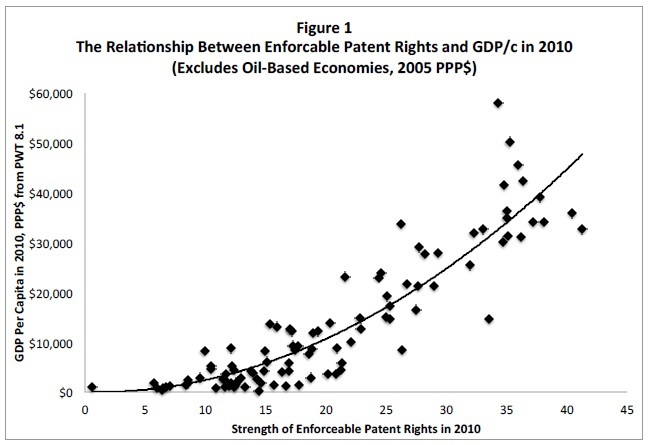
\includegraphics[scale=0.75]{patents_and_gdp.jpg}
\end{center}
\caption{Veza između striktnosti očuvanja patenata zemalja i njihovog bruto domaćeg proizvoda.}
\label{fig:pat_gdp}
\end{figure}

\subsection{Moralni aspekt}
\label{subsec:morala_sam}

\section{Sprovođenje u Srbiji}
\label{sec:srb}

\section{Zaključak}
\label{sec:zakljucak}

Ovde pišem zaključak. 
Ovde pišem zaključak. 
Ovde pišem zaključak. 
Ovde pišem zaključak. 
Ovde pišem zaključak. 
Ovde pišem zaključak. 
Ovde pišem zaključak. 
Ovde pišem zaključak. 
Ovde pišem zaključak. 
Ovde pišem zaključak. 
Ovde pišem zaključak. 
Ovde pišem zaključak. 


\addcontentsline{toc}{section}{Literatura}
\appendix
\bibliography{seminarski} 
\bibliographystyle{plain}

\appendix
\section{Dodatak}
Ovde pišem dodatne stvari, ukoliko za time ima potrebe.
Ovde pišem dodatne stvari, ukoliko za time ima potrebe.
Ovde pišem dodatne stvari, ukoliko za time ima potrebe.
Ovde pišem dodatne stvari, ukoliko za time ima potrebe.
Ovde pišem dodatne stvari, ukoliko za time ima potrebe.


\end{document}
